%%%%%%%%%%%%%%%%%%%%%%%%%%%%%%%%%%%%%%%%%%%%%%%%%%%%%%%%%%%%%%%%%%%%%
% LaTeX Template: Relatório de LSD
% Ano Letivo: 2026/2027
% Disciplina: Lógica e Sistemas Digitais
% Docente: Pedro Miguens Matutino
% Autor: Pedro Miguens Matutino
%%%%%%%%%%%%%%%%%%%%%%%%%%%%%%%%%%%%%%%%%%%%%%%%%%%%%%%%%%%%%%%%%%%%%%
\documentclass[12pt]{article}

\usepackage[a4paper]{geometry}
\usepackage[T1]{fontenc}
\usepackage[utf8]{inputenc}
\usepackage[portuguese]{babel}

\usepackage{graphicx, wrapfig, subcaption, setspace, booktabs, longtable}
\usepackage[font=small, labelfont=bf]{caption}
\usepackage{listings}
\usepackage{tocloft}
\usepackage{url, lipsum}
\usepackage{hyperref}

\usepackage{tikz}
\usetikzlibrary{karnaugh}

\usepackage{xcolor}
\usepackage{amsmath}
\usepackage{amsfonts}
\usepackage{amssymb}

\usepackage{enumitem}
\usepackage{algorithm}

\usepackage{fancyhdr}

%-------------------------------------------------------------------------------
% Definição da listagens de VHDL  ----------------------------------------------
%-------------------------------------------------------------------------------
\definecolor{vhdlkeyword}{RGB}{0,70,140}
\definecolor{vhdltype}{RGB}{130,0,80}
\definecolor{vhdlcomment}{RGB}{0.07,0.65,0.28}
\definecolor{vhdlstring}{RGB}{160,80,0}

\lstdefinelanguage{VHDL}{
    morekeywords={
        library,use,all,entity,is,port,in,out,inout,
        architecture,of,begin,end,signal,constant,
        component,configuration,package,body,
        process,wait,on,until,for,
        if,then,else,elsif,case,when,
        loop,while,next,exit,
        generate,generic,map,
        function,procedure,return,
        variable,file,type,subtype,record,array,
        downto,to,range,
        assert,report,severity,
        after,transport,inertial,
        with,select,others
    },
    morekeywords=[2]{
        std_logic,std_logic_vector,
        bit,bit_vector,
        integer,natural,positive,
        boolean,character,string,time
    },
    sensitive=true,
    morecomment=[l]--,
    morestring=[b]"
}

\lstset{
    language=VHDL,
    basicstyle=\ttfamily\tiny,
    keywordstyle=\color{vhdlkeyword}\bfseries,
    keywordstyle=[2]\color{vhdltype},
    commentstyle=\color{vhdlcomment}\itshape,
    stringstyle=\color{vhdlstring},
    numbers=left,
    numberstyle=\tiny\color{gray},
    numbersep=8pt,
    frame=single,
    breaklines=true,
    showstringspaces=false
}




\addto\captionsportuguese{
    \renewcommand{\figurename}{Figura}
    \renewcommand{\tablename}{Tabela}
    \renewcommand{\listfigurename}{Lista de Figuras}
    \renewcommand{\listtablename}{Lista de Tabelas}
}

% List of Figures
\renewcommand{\cftfigpresnum}{Figura~}
\renewcommand{\cftfigaftersnum}{}
\setlength{\cftfignumwidth}{5em}

% List of Tables
\renewcommand{\cfttabpresnum}{Tabela~}
\renewcommand{\cfttabaftersnum}{}
\setlength{\cfttabnumwidth}{5em}

% List of VHDL listings
\makeatletter
\renewcommand{\lstlistingname}{VHDL}
\renewcommand{\lstlistlistingname}{Lista de VHDL}
\renewcommand{\l@lstlisting}[2]{%
  \@dottedtocline{1}{0em}{5em}{VHDL~#1}{#2}%
}
\makeatother

%-------------------------------------------------------------------------------
% Início do documento ----------------------------------------------------------
%-------------------------------------------------------------------------------
 \begin{document}

% Parametros do documento
\tikzset{
  grp/.style n args={3}{
    draw=#1,fill=#1!30,
    minimum width=#2\kmunitlength,
    minimum height=#3\kmunitlength,
    rounded corners=0.2\kmunitlength,
    fill opacity=0.6,
    rectangle}
}
   
%-------------------------------------------------------------------------------
% Início da capa de rosto ------------------------------------------------------
%-------------------------------------------------------------------------------
\begin{titlepage}
    \begin{flushleft}
      \hspace{-1.5cm}
      
\includegraphics[height=3.5cm]{figures/01_ISEL-Logotipo-RGB_Horizontal-Compacto-900.png}

      Licenciatura em Engenharia Informática e de Computadores
    \end{flushleft}

    \vspace{2.0cm}

    \begin{center}
      \textbf{Lógica e Sistemas Digitais}

      2026 / 2027  inverno

      \vspace{0.5cm}
      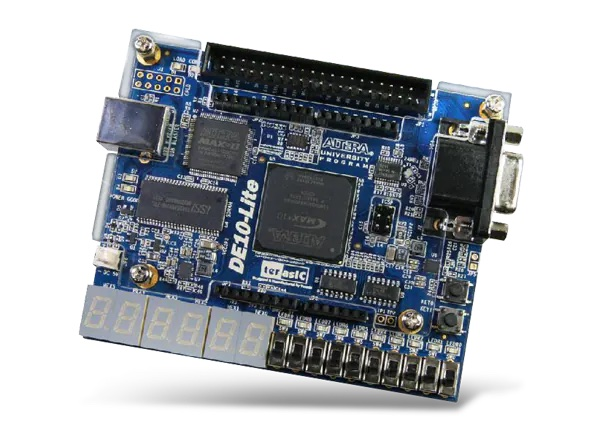
\includegraphics[width=6cm]{figures/de10-lite.jpg}\\
      \vspace{0.5cm}
      
      \Large {Relatório do \\Trabalho Laboratorial 2}\\
      
      \textbf{Circuitos Aritméticos e Lógicos}
    \end{center}

    \vspace{1.0cm}

Trabalho realizado por:

\begin{itemize}[label={}]
    \item 56012 -- João Ferreira
    \item 56010 -- André Granja
\end{itemize}

\vspace{0.5cm}
Turma: \\

Docente: Pedro Miguens

\date{}

\end{titlepage}
%-------------------------------------------------------------------------------
% Fim da capa de rosto ---------------------------------------------------------
%-------------------------------------------------------------------------------

%-------------------------------------------------------------------------------
% Parâmetros do cabeçalho e rodapé
%-------------------------------------------------------------------------------
\renewcommand{\headrulewidth}{1pt}
\definecolor{iselcolor}{rgb}{0.941,0.275 , 0.157} 
\definecolor{isel_beringela}{rgb}{0.37,0.08, 0.22} 
\renewcommand{\headrule}{\hbox to\headwidth{%
  \color{iselcolor}\leaders\hrule height \headrulewidth\hfill}}
\setlength\headheight{70pt}

\pagestyle{fancy}
\fancyhead{} % clear all header fields
\fancyhead[LO]{
\includegraphics[width=2.5cm]{figures/01_ISEL-Logotipo-RGB_Horizontal-Compacto-900.png}}
\fancyhead[RO]{\footnotesize Lógica e Sistemas Digitais 2026/2027 inverno \\ Trabalho Laboratorial 2}


%-------------------------------------------------------------------------------
% Indice, lista de figuras, lista de tabelas e lista de códigos
%-------------------------------------------------------------------------------
\setcounter{page}{1}
\pagenumbering{roman} % Roman page numbers
\tableofcontents
\clearpage
\addcontentsline{toc}{section}{\protect\numberline{}Lista de Figuras}
\listoffigures
\addcontentsline{toc}{section}{\protect\numberline{}Lista de Tabelas}
\listoftables
\addcontentsline{toc}{section}{\protect\numberline{}Lista de VHDL}
\lstlistoflistings
\clearpage

%-------------------------------------------------------------------------------
% Corpo do relatório
%-------------------------------------------------------------------------------
\pagenumbering{arabic} % Arabic/Indic page numbers
\setcounter{page}{1}

\section{Objetivo}
O objetivo deste trabalho é projetar uma unidade aritmética e lógica (ALU)
de 4 bits em VHDL estrutural, simular o circuito através de um testbench e
implementá-lo na placa DE10-Lite. A ALU deve executar quatro operações
aritméticas, duas operações lógicas e dois deslocamentos, produzindo também
as flags Carry/Borrow, Overflow, Zero, Greater or Equal e Below or Equal.

\section{Descrição do Circuito a Projetar}
As entradas da ALU são os operandos de 4 bits $X$ e $Y$, a operação de
3 bits $OP$ e o carry/borrow de entrada $CBi$. O resultado $R$ tem 4 bits.
As operações aritméticas são $X+Y+CBi$, $X-Y-CBi$, $Y+CBi$ e
$-Y-CBi$. As operações lógicas são AND e NAND. Para além destas,
existem os deslocamentos LSL de $X$ por $Y(1..0)$ posições e ASR de $X$
por uma posição.

As flags CBo e OV indicam, respetivamente, carry/borrow e overflow com
sinal. A flag Z indica resultado nulo. As flags GE e BE correspondem às
comparações $X \geq Y+CBi$ em complemento para dois e
$X \leq Y+CBi$ como naturais.

\section{Desenvolvimento do Projeto}
O projeto foi dividido em módulos independentes. A unidade aritmética do
LABc foi reutilizada, incluindo o somador completo, o somador de 4 bits,
o somador/subtrator e a unidade de flags. Foram acrescentados os módulos
Xor0, Logic Module, Decode OP, MUX e a unidade final de flags.

\subsection{Diagrama de blocos}
O decoder transforma $OP$ nos sinais de controlo internos. O bloco Xor0
seleciona $X$ ou zero para a entrada $A$ da unidade aritmética. Em
paralelo, o Logic Module calcula o resultado lógico ou de deslocamento.
Por fim, o MUX seleciona o resultado aritmético ou lógico.
\begin{figure}[!h]
	\centering
	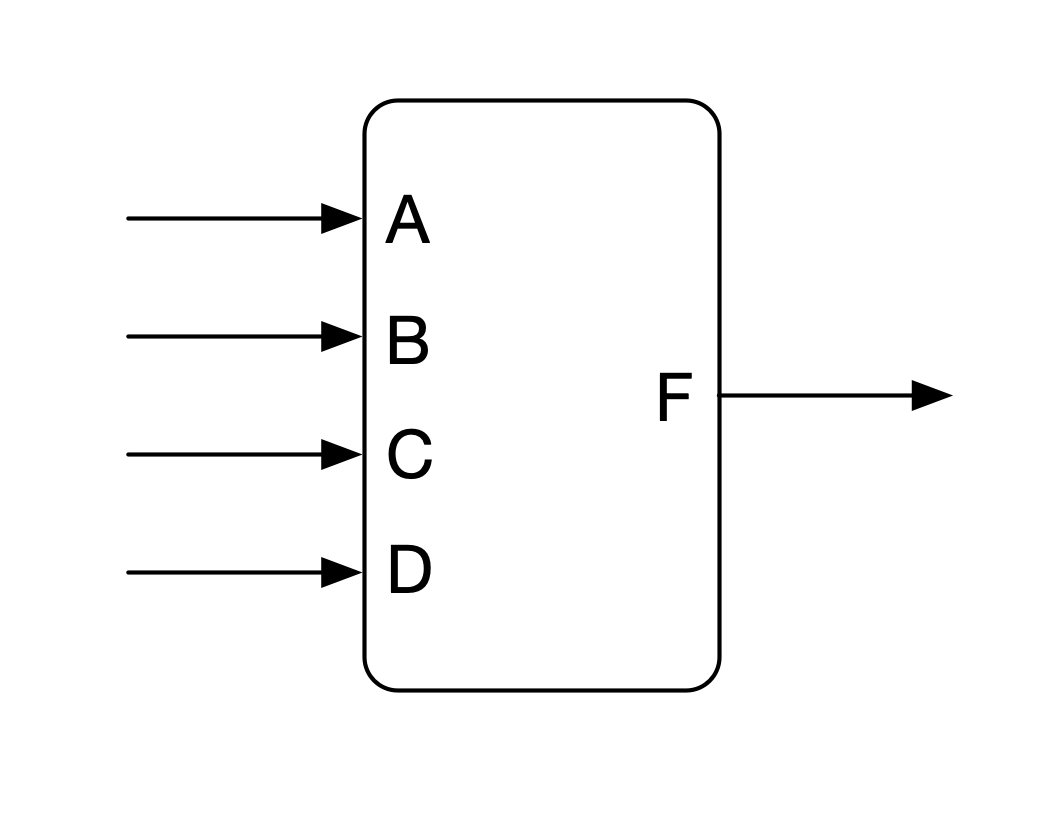
\includegraphics[width=0.5\textwidth]{figures/DiagramaBlocos.png}
	\caption{Diagrama de blocos da ALU}
	\centering
	\label{fig:diagramablocos}
\end{figure}

\subsection{Funções lógicas dos circuitos}
Para o LSL, o valor de $Y(1..0)$ determina o número de deslocamentos.
Os zeros são introduzidos nos bits menos significativos e o último bit
retirado de $X$ é usado como carry lógico. No ASR, o bit de sinal é
replicado e $X(0)$ é usado como carry.

Os ficheiros VHDL foram descritos com uma entidade por ficheiro. A
entidade de topo é estrutural e liga todos os módulos através de
instanciações e port maps.


\section{Resultados e Discussão}
Foi criada uma tabela de resultados teóricos para as 20 combinações do
enunciado e para quatro combinações adicionais. Os valores encontram-se
em \texttt{ANEXO\_A\_RESULTADOS.md}. Nas operações em que uma flag não
tem significado, essa flag foi marcada com ``-''.

\subsection{Simulação}
O testbench verifica as 24 linhas do Anexo A e executa ainda um teste
exaustivo de 4096 combinações, correspondente a todos os valores possíveis
de $X$, $Y$, $OP$ e $CBi$. A compilação e a simulação foram executadas no
ModelSim/QuestaSim através do script \texttt{simulate.do}. Não foram
detetados erros no testbench.

\subsection{Teste}
A implementação na DE10-Lite utiliza SW[3..0] para $X$, SW[7..4] para
$Y$, SW[9..8] para $OP[1..0]$, KEY[0] para $OP[2]$ e KEY[1] para $CBi$.
Os LEDs apresentam o resultado e as cinco flags. Os resultados
experimentais da placa devem ser preenchidos após a programação física.

\section{Conclusão} 
Foi desenvolvida uma ALU de 4 bits em VHDL estrutural, reutilizando a
unidade aritmética do LABc e acrescentando os módulos lógicos, de controlo,
MUX e flags. A simulação compilou sem erros e o testbench confirmou as
24 combinações previstas e as 4096 combinações exaustivas. A validação
experimental na DE10-Lite deverá ser concluída após a programação da placa.

%-------------------------------------------------------------------------------
% REFERENCES
%-------------------------------------------------------------------------------
\clearpage
%\section*{Referências}
\addcontentsline{toc}{section}{\protect\numberline{}Referências}
\begin{thebibliography}{9}
\bibitem{guiaQuartus}
Pedro Miguens Matutino, Sérgio André \emph{Guia de Instalação do Quartus Prime Lite Edition 20.1.1.720}, 2022, ISEL.
\bibitem{de10liteManual}
Terasic \emph{DE10-lite User Manual}, 2020, Terasic.
\end{thebibliography}


\clearpage
\appendix
\section{Resultados teóricos do Anexo A}
Os valores seguintes correspondem aos resultados teóricos das combinações
do enunciado e das quatro combinações adicionais definidas pelo grupo.
Nas flags sem significado, utiliza-se ``--''.

\begin{center}
\scriptsize
\setlength{\tabcolsep}{2pt}
\begin{longtable}{c c c c r r c c r r c c r r c c c}
\caption{Resultados teóricos do Anexo A}\\
\toprule
\# & OP & CBi & X & X(N) & X(Z) & Y & Y(N) & Y(Z) & R & R(N) & R(Z) & CBo & OV & Z & GE & BE\\
\midrule
\endfirsthead
\toprule
\# & OP & CBi & X & X(N) & X(Z) & Y & Y(N) & Y(Z) & R & R(N) & R(Z) & CBo & OV & Z & GE & BE\\
\midrule
\endhead
1&000&0&0000&0&0&1111&15&-1&1111&15&-1&0&0&0&--&--\\
2&000&1&0000&0&0&1111&15&-1&0000&0&0&1&0&1&--&--\\
3&000&1&0101&5&5&1000&8&-8&1110&14&-2&0&0&0&--&--\\
4&000&1&1111&15&-1&1010&10&-6&1010&10&-6&1&0&0&--&--\\
5&001&1&0000&0&0&1111&15&-1&1111&15&-1&1&0&0&1&1\\
6&001&1&0001&1&1&0101&5&5&1011&11&-5&1&0&0&0&1\\
7&001&1&1010&10&-6&0111&7&7&0010&2&2&0&1&0&0&0\\
8&010&0&--&--&--&0001&1&1&0001&1&1&0&0&0&--&--\\
9&010&1&--&--&--&0001&1&1&0010&2&2&0&0&0&--&--\\
10&010&1&--&--&--&0111&7&7&1000&8&-8&0&1&0&--&--\\
11&010&1&--&--&--&1111&15&-1&0000&0&0&1&0&1&--&--\\
12&011&0&--&--&--&0000&0&0&0000&0&0&0&0&1&--&--\\
13&011&0&--&--&--&1000&8&-8&1000&8&-8&1&1&0&--&--\\
14&011&1&--&--&--&0110&6&6&1001&9&-7&1&0&0&--&--\\
15&011&1&--&--&--&1000&8&-8&0111&7&7&1&0&0&--&--\\
16&100&1&0001&1&1&1100&12&-4&0000&0&0&--&--&1&--&--\\
17&100&0&1101&13&-3&1001&9&-7&1001&9&-7&--&--&0&--&--\\
18&101&0&1010&10&-6&1110&14&-2&0101&5&5&--&--&0&--&--\\
19&110&0&1001&9&-7&0110&6&6&0100&4&4&0&--&0&--&--\\
20&111&1&1111&15&-1&--&--&--&1111&15&-1&1&--&0&--&--\\
21&000&1&0111&7&7&0111&7&7&1111&15&-1&0&1&0&--&--\\
22&001&0&1000&8&-8&0001&1&1&0111&7&7&0&1&0&0&0\\
23&100&0&1010&10&-6&1100&12&-4&1000&8&-8&--&--&0&--&--\\
24&110&0&0011&3&3&0010&2&2&1100&12&-4&0&--&0&--&--\\
\bottomrule
\end{longtable}
\end{center}

\section{VHDL}
% Inserção de ficheiro de descrição hardware
\lstinputlisting[
    inputencoding=latin1,
    caption={Entidade de topo da ALU},
    label={vhdl:alu}
]{../../alu.vhd}

O testbench completo encontra-se no ficheiro \texttt{alu\_tb.vhd} entregue
com o projeto.


\clearpage
\section{Atribuição de Pinos}

\renewcommand{\arraystretch}{1.5}
\begin{table}[h]\footnotesize
	\caption{Atribuição lógica de entradas e saídas na DE10-Lite}
  \centering
	\begin{tabular}{|l|c|}
	\hline
	\textbf{Sinal ALU} & \textbf{Placa} \\ \hline\hline
	X[3..0] & SW[3..0]  \\ 
	Y[3..0] & SW[7..4] \\
	OP[1..0] & SW[9..8] \\
	OP[2] & KEY[0] \\
	CBi & KEY[1] \\ \hline \hline
	R[3..0] & LEDR[3..0] \\
CBo & LEDR[4] \\
	OV & LEDR[5] \\
	Z & LEDR[6] \\
	GE & LEDR[7] \\
	BE & LEDR[8] \\
	\hline
	\end{tabular}
	
	\label{tab:pinos}
\end{table}

\end{document}